% !TeX encoding = UTF-8
% !TeX root = vldb2018.tex
% !TeX spellcheck = en_US

\begin{figure*}%
	\captionsetup[subfigure]{justification=centering}
	\null\hfill
	\begin{subfigure}[b]{1.4cm}
		\centering
		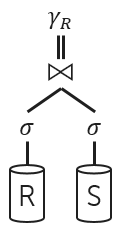
\includegraphics[scale=0.6]{figures/QP-Normal.png}
		\caption{Normal \phantom{Onetime}}
		\label{fig:QueryProcessing:normal}
	\end{subfigure}
	\hfill
	\begin{subfigure}[b]{1.5cm}
		\centering
		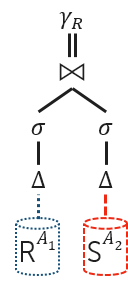
\includegraphics[scale=0.6]{figures/QP-Early.png}
		\caption{Early\\Onetime}
		\label{fig:QueryProcessing:early}
	\end{subfigure}
	\hfill
	\begin{subfigure}[b]{1.5cm}
		\centering
		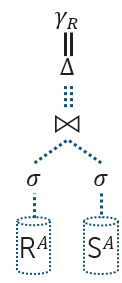
\includegraphics[scale=0.6]{figures/QP-Late1.png}
		\caption{Late\\Onetime 1}
		\label{fig:QueryProcessing:late1}
	\end{subfigure}
	\hfill
	\begin{subfigure}[b]{1.5cm}
		\centering
		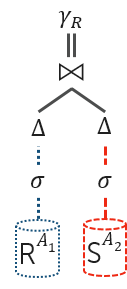
\includegraphics[scale=0.6]{figures/QP-Late2.png}
		\caption{Late\\Onetime 2}
		\label{fig:QueryProcessing:late2}
	\end{subfigure}
	\hfill
	\begin{subfigure}[b]{2cm}
		\centering
		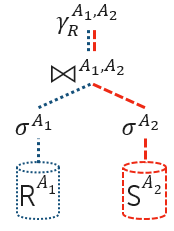
\includegraphics[scale=0.6]{figures/QP-Continuous.png}
		\caption{Continuous \phantom{Onetime}}
		\label{fig:QueryProcessing:continuous}
	\end{subfigure}
	\hfill
	\begin{subfigure}[b]{2.5cm}
		\centering
		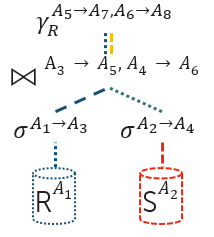
\includegraphics[scale=0.6]{figures/QP-Continuous-Reencoding.png}
		\caption{Continuous With Reencoding}
		\label{fig:QueryProcessing:reencoding}
	\end{subfigure}
	\hfill\null
	\vspace{-0.3cm}
	\caption{Illustration of the query processing variants. \(\Delta\) is a dedicated check-and-decode operator. Different \(A\)s are indicated via superscripts at the columns and operators, and via different colors and line decorations. Reencoding is indicated as \(A_1 \rightarrow A_2\).}%
	\label{fig:QueryProcessing}%
	\vspace{-0.3cm}
\end{figure*}


\section{On-the-fly Error Detection}
\label{sec:ResilientQueryProcessing}




On\=the\=fly error detection during query processing becomes now possible for both state\=of\=the\=art processing models of column\=at\=a\=time~\cite{DBLP:journals/ftdb/AbadiBHIM13,DBLP:journals/debu/IdreosGNMMK12} and vector\=at\=a\=time~\cite{DBLP:conf/icde/ZukowskiWB12} with our hardened storage concept. There are two reasons: (i) the column structure is unchanged, only the data width is increased and (ii) the values are multiplied by \(A\) and can thus be processed as before. 

\subsection{Error Detection Opportunities}

Basically, there are three opportunities for on\=the\=fly error detection as shown in \Cref{fig:QueryProcessing}, whereby \Cref{fig:QueryProcessing:normal} represents an example query execution plan (QEP) without any hardened data. In this QEP, data from two columns \(R\) and \(S\) is filtered, the results are joined, and finally grouped by column \(R\). We use this QEP, to describe our three detection possibilities during query processing. 

\textbf{Early Onetime Detection: }
As a first possibility, error detection happens only once, when touching data the very first time in the base columns (\Cref{fig:QueryProcessing:early}). For that, we introduce the \emph{detect\=and\=decode} operator \(\Delta\) taking as input a column containing hardened data and outputing a column containing the decoded data. \(\Delta\) is put before any other operator in the QEP. The physical realization of \(\Delta\) is based on a regular column scan\=operator conducting detection and decoding based on the formulas presented in Section~\ref{sec:ANCodingImprovements}. However, the disadvantage is that bit flips during the remaining query processing are not detected.

\textbf{Late Onetime Detection: }
Second, since AN coding allows arbitrary operations directly on hardened data, detection may take place in a late stage of a QEP. For instance, a hardened column can be filtered just by encoding the filter predicate with the same \(A\) the input columns are hardened with. Thus, our \emph{detect\=and\=decode} \(\Delta\) can be placed in the QEP at a point, where there are still sufficiently many tuples left for bit flip detection, e.g. before a group-by as in \Cref{fig:QueryProcessing:late1}. Operators taking multiple inputs, like joins, may encounter differently encoded inputs so that \(\Delta\) must be placed before these (\Cref{fig:QueryProcessing:late2}, \Cref{sec:AdjustmentsForContinuous} provides further details). However, the disadvantage is that bit flips are only detected at a single point and errors are propagated through the QEP. 


\textbf{Continuous Detection: }
Thus, we have to integrate bit flip detection into each and every physical operator (\Cref{fig:QueryProcessing:continuous}). This is conceptually the best solution, because bit flips are quickly detected and \(\Delta\) becomes superfluous. By that, each and every value is checked for bit flips in the columns of base tables and intermediate results.

\subsection{Adjustments for Continuous Detection}
\label{sec:AdjustmentsForContinuous}

We now focus on necessary adjustments to the query processing to realize the continuous error detection approach. 

\textbf{Error Detection Primitives for Physical Operators:}
Each physical query operator has to be adjusted to include appropriate AN coding detection primitives. We do this with a vector storing the array position of corrupted values per column. Of course, this error vector can also be affected by bit flips, so we harden it with AN coding, too. 
%In reality, an error correction activity for each detected error has to be triggered and we return to this aspect in Section~\ref{sec:Correction}. 
Further adjustments are exemplarily described for a \texttt{filter scan} operator on signed integers, as shown in \Cref{alg:continuous:filter}. For reasons of better traceability, the algorithm description is conceptually based on MonetDB primitives using their BAT data structures for columns~\cite{DBLP:journals/vldb/BonczK99}. The operator takes two inputs: (i) a single hardened input BAT and (ii) a hardened predicate (\emph{pred}\(^*\)). To provide a full\=fledged example, assume that (i) both head and tail of the input BAT are non\=virtual and encoded with different \(A\)s and (ii) the operator returns a hardened output BAT and two error vectors. First, the operator initializes the error vectors (lines 1 and 2). Variable \texttt{pos} (lines 3 and 15) is used to keep track of the position in the input BAT, so that we are able to store the error position within the input BAT. When iterating over head and tail they are first decoded (lines 5 and 6) and then tested according to \Cref{eq:newvalidate:max,eq:newvalidate:min} (lines 7 and 10). Upon detection of an error, the hardened position is stored in the appropriate error vector (lines 8 and 11). If the tail value is assumed to be valid, the filter is evaluated (line 12) and if it matches, the hardened column value is appended to the output BAT (line 13). Likewise, this pattern can be applied to all other physical operators, whereas the number of error vectors varies depending on the number of input columns.


\begin{algorithm}[t]
\caption{\texttt{Filter scan} for continuous error detection, having head and tail hardened with different \(A\)s and reencoding its output. \(^*\) denotes hardened values and BATs. Subscript \(_h\) and \(_t\) denote head and tail, respectively.}
\label{alg:continuous:filter}
\begin{algorithmic}[1]
\Require \(B_\text{in}^*\)                                     \Comment{hardened input BAT}
\Require \(A_h,A_h^{-1},A_t,A_t^{-1}\)                         \Comment{AN coding parameters}
\Require \(A_h^\prime,A_t^\prime\)                             \Comment{Reencoding parameters}
\Require \(A_\text{pos}\)                                      \Comment{Error position hardening parameter}
\Require \(d_{h,\text{max}},d_{t,\text{max}}\)                 \Comment{largest unencoded values for \(B^*_\text{in}\)}
\Require \(d_{h,\text{min}},d_{t,\text{min}}\)                 \Comment{smallest unencoded value for \(B^*_\text{in}\)}
\Require \(\circ\in\{<,\leq,=,\not=,\geq,>\}\)                 \Comment{comparison operator}
\Require \emph{pred}\(^*\)                                     \Comment{predicate encoded with \(A_t\)}
\Ensure \(B^*_\text{out}\)                                     \Comment{result BAT (same \(A\) as \(B_\text{in}^*\))}
\Ensure \(v_h, v_t\)                                           \Comment{error bit vectors for \textbf{h}ead and \textbf{t}ail}
\State \(v_h.initialize()\)                                    \Comment{allocate memory for \(v_h\)}%
                                                                   \label{lst:line:vh:init}
\State \(v_t.initialize()\)                                    \Comment{allocate memory for \(v_t\)}%
                                                                   \label{lst:line:vt:init}
\State pos \(\gets 0\)                                             \label{lst:line:pos:init}
\ForEach{(head\(^*\), tail\(^*\)) \(\in B_\text{in}^*\)}           \label{lst:line:for1}
	\State \(h \gets \text{head\(^*\)} * A_h^{-1}\)                \label{lst:line:h}
	\State \(t \gets \text{tail\(^*\)} * A_t^{-1}\)                \label{lst:line:t}
	\If{\(h < d_{h,\text{min}} \Or h > d_{h,\text{max}}\)}         \label{lst:line:if1}
		\State \(v_h.append(pos * A_\text{pos})\)                  \label{lst:line:vh:set}
	\EndIf                                                         \label{lst:line:endif1}
	\If{\(t < d_{t,\text{min}} \Or t > d_{t,\text{max}}\)}         \label{lst:line:if2}
		\State \(v_t.append(pos * A_\text{pos})\)                  \label{lst:line:vt:set}
	\ElsIf{tail\(^*\) \(\circ\) \emph{pred}\(^*\)}                 \label{lst:line:elseif2}
		\State append (\(h * A_h^\prime\), \(t * A_t^\prime\)) to \(B^*_\text{out}\)   \label{lst:line:append}
	\EndIf                                                         \label{lst:line:endif2}
	\State pos \(\gets\) pos \(+1\)                                \label{lst:line:pos:inc}
\EndFor                                                            \label{lst:line:endfor1}
\end{algorithmic}
\end{algorithm}

%Aside from this adjustment for error detection primitives, the physical operators may have to work on larger input value bit widths. However, this is a minor adjustment. 

\textbf{Physical Operations with Different \(A\)s:}
\Cref{tab:optimalAs} shows that there are different super \(A\)s for different data widths. Consequently, base columns will be hardened with different \(A\)s. In \Cref{fig:QueryProcessing} different \(A\)s are indicated by superscripts at data and operators and by different line types and colors between operators. Columns with different \(A\)s are a challenge for binary operations like joins (see \Cref{fig:QueryProcessing:continuous}). There, for different \(A\)s it holds that \((d \cdot A_1) \neq (d \cdot A_2), ~ A_1 \neq A_2\) and an equi-join would at most produce false positives, when \(d_1\cdot A_1=d_2\cdot A_2, ~ d_1 \neq d_2\). To produce correct results, binary operators have to adapt one of the inputs (hardened with \(A_1\)) to match the other's \(A_2\) by multiplying the factor \(A_1^{-1}\cdot A_2\) onto each hardened value of the first input column, or \(A_1\cdot A_2^{-1}\) onto the second. Optionally, the decoded value, which is computed for error detection and resides in a CPU register, could be multiplied by \(A_2\) only, as well. As a side effect, each operator may well harden or soften the data on-the-fly (\Cref{fig:QueryProcessing:reencoding}), called reencoding. This can, e.g., reduce the data width for intermediate results or prepare the data for the following operator (cooperative operators as introduced in~\cite{DBLP:conf/cidr/KissingerSHL13}). Consequently, it allows to adjust space requirements against reliability, i.e., multi\=bit flip detection capabilities. Reencoding is actually the same as the adaptation described for the join operator. In \Cref{fig:QueryProcessing:reencoding}, each operator reencodes its input with a new \(A\), indicated as \(A_x\rightarrow A_y\). Generally, this reencoding is a very interesting property as will be shown in the evaluation. 



\textbf{Handling of Intermediate Results:}
Because all operations can directly work on hardened data and each operator passes its hardened results to the next operator, the intermediate results are automatically hardened. There is only one special feature in column stores, namely, virtual IDs can sometimes be materialized during the query processing~\cite{DBLP:journals/ftdb/AbadiBHIM13,DBLP:journals/debu/IdreosGNMMK12}. In order to detect errors during the further processing of these virtual IDs, these IDs are automatically hardened during their generation. Differently encoded IDs can be handled as indicated above for the join.

\textbf{Bit Flip Detection in ALU Operations:}
As described in Section~\ref{sec:ErrorCoding}, AN coding allows to detect errors in certain operations of a CPU's ALU (arithmetic logic unit), which performs arithmetic, comparison and logic operations. For arithmetic operations like \(+,-,/,\dots\) (cf. \Cref{eq:ANPlusMinus,eq:ANMulUnenc,eq:ANMulOK,eq:ANDivUnenc,eq:ANDivOK}), the result can be immediately checked by multiplying with the respective \(A\)'s inverse. The checks must be anchored in the corresponding physical operators, as already described.

Error detection for comparison operations like \(<,\leq,=,\dots\) (cf. \Cref{eq:ANCompare}) is much more challenging, since comparisons are required for the detection itself. We could use a technique similar to branch-avoidance by replacing the comparison with an array access, as depicted in \Cref{fig:ANComparisonFix}. Suppose that for each comparison operator there is an infinitely large array of boolean values:
\[
	a_\text{Op}[i]\in\{\top,\bot\}, ~ \text{Op}\in\{<,\leq,\dots\}, ~ i\in\{-\infty\dots0\dots\infty\}.
\]
The difference of the two operands yields the position in the array, where we find the boolean value representing the result of the original comparison operation. For instance, \Cref{fig:ANComparisonFix:Equal} illustrates the array contents for the equality comparison. There, we compute the difference of the two operands \(c_2-c_1\) and the array contains only one \texttt{true} value at position zero, since \(c_2=c_1 \Leftrightarrow c_2-c_1=0\). Likewise, for '$<$' comparison (\Cref{fig:ANComparisonFix:Less}), we find \texttt{true} only for \(i>0\) and for '$\leq$' \texttt{true} is at all \(i\geq0\). However, infinite arrays can not be stored in memory and their contents would have to be verified at runtime as well.

\begin{figure}%
	\null\hfill
	\begin{subfigure}[t]{1in}
		\centering
		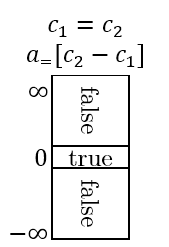
\includegraphics[width=.5in]{figures/ComparisonEquality.png}
		\caption{Equal}
		\label{fig:ANComparisonFix:Equal}
	\end{subfigure}
	\hfill
	\begin{subfigure}[t]{1in}
		\centering
		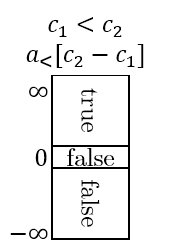
\includegraphics[width=.5in]{figures/ComparisonLessThan.png}
		\caption{Less-Than}
		\label{fig:ANComparisonFix:Less}
	\end{subfigure}
	\hfill
	\begin{subfigure}[t]{1in}
		\centering
		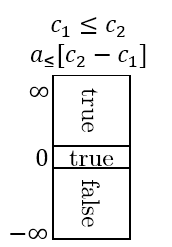
\includegraphics[width=.5in]{figures/ComparisonLessEqual.png}
		\caption{Less-or-Equal}
		\label{fig:ANComparisonFix:LessEqual}
	\end{subfigure}
	\hfill\null
	\vspace{-0.3cm}
	\caption{Replacing comparison by access to a boolean array.}%
	\label{fig:ANComparisonFix}%
	\vspace{-0.4cm}
\end{figure}


Consequently, errors in logic operations (\(\&, \|, \oplus, \neg\)) cannot be detected solely by AN coding and bit operations like AND-ing, OR-ing, XOR-ing, or inverting all bits produce \emph{invalid} code words. By that, these operations must be protected in another way. Therefore, we assume \emph{reliable} comparison and logic operations. Both areas must be considered separately in future work.

\textbf{Vectorization:}
The array-like hardened storage of columns, where only values of the very same data type are stored, allows to use vectorization (SIMD) instructions~\cite{DBLP:conf/icde/ZukowskiHNB06,willhalm2013vectorizing}. Our improved AN coding requires only multiplication and comparison, which are well supported as SIMD instructions in virtually all modern processors. Consequently, for code word widths which fit into native SIMD registers, our \emph{AHEAD} approach can be well combined with vectorizable physical operators like filter or aggregation. Willhalm et al. show how data with bit widths from 1 to 32 bits is aligned in SIMD registers to be processable, even with complex predicates and with special optimizations for each bit case~\cite{willhalm2013vectorizing}. After their alignment step, multiplication and comparison instructions for AN coding operations can be included. There are, however, some peculiarities with SIMD operations. As of now, instruction sets like Streaming SIMD Extensions (all variants until SSE4.2) and Advanced Vector Extensions 1 \& 2 do not support unsigned integer comparison, which must be emulated with 2 operations. For instance, for the unsigned ``\(>\)'' comparison in SSE4.2, instead of a single
\begin{flalign*}
& v_> = \texttt{\_mm\_cmpgt\_epu(vector(} d_0,d_1,\dots \texttt{), vector(} d_\text{max} \texttt{))}, &
\end{flalign*}
the following is required:
\begin{flalign*}
& v_\text{tmp} = \texttt{\_mm\_max\_epu(vector(} d_0,d_1,\dots \texttt{), vector(} d_\text{max} + 1 \texttt{))} & \\
& v_> = \texttt{\_mm\_cmpeq\_epi(} v_\text{tmp} \texttt{, vector(} d_0,d_1,\dots \texttt{)} &
\end{flalign*}
Afterwards, the result of the comparison can be translated into an integer using one of the \texttt{\_mm\_movemask} instruction variants. AVX-512 is supposed to provide the comparisons natively and some operations even immediately return an appropriate mask, so instead of three instructions, a single one suffices -- at least from a source code perspective.

%\subsection{Handling of Detected Bit Flips}
%\label{sec:Correction}
%
%So far, we have only been concerned with the continuous detection of bit flips during query processing. However, our \emph{AHEAD} approach also allows initial and straightforward error correction capabilities in a fine-grained way. Generally, we are currently able to detect and distinguish two kinds of errors: (i) bit flips during arithmetics and (ii) input data errors. For the latter case, however, we cannot distinguish between bit flips in main memory or those induced in interconnects. When we detect a faulty code word in the inputs, we can retransmit it, possibly several times, to correct errors induced during transmission. If we get a valid code word, processing can continue with this correct code word. If we get an invalid code word, we can assume that bits are flipped in main memory and then require an appropriate technique for error correction.
%
%Since errors during arithmetic operations are detected separately, we can also correct them separately. In principle, the operands are correct, only the arithmetic operation provides errors. To correct these errors, the single arithmetic operation can also be performed repeatedly until we get a valid resulting code word. Nevertheless, the presented error correction approaches are straightforward and should show the potential of our approach. With our \emph{AHEAD} approach, we can detect bit flips on value granularity and can find out where the error occurred. This allows us to initiate specific techniques for correction. The development of suitable techniques and the integration is subject to future work.
%




%\textbf{Ch\textsubscript{\cntincarabic{ChallengesCounter}}) Intermediate Results:}
%On the one hand, intermediate result are potentially evicted from the CPU cache to main memory. On the other hand, they may contain newly generated data, e.g. materialized OIDs from a BAT filter scan, or aggregates. A major drawback of Early Onetime Detection is, that \emph{any} bit flips in any intermediate results stay undetected. Late Onetime only mitigates this, as \(\Delta\) is further up in the query plan (cf. \Cref{fig:QueryProcessing:early,fig:QueryProcessing:late1}). In contrast, Continuous Detection does not produce unencoded intermediate results. By that, each and every value stays hardened and can be checked for bit flips. \inlinetodo{early and late do not produce hardened OIDs in intermediate results}
%
%
%
%
%
%

%
%

%
%
%
%
%\textbf{Ch\textsubscript{\cntincarabic{ChallengesCounter}}) Handling Detected Bit Flips:}
%For DRAM errors, we only set the error bits in the respective bit vectors and attempt no correction, yet. Soft errors during ALU operations do not modify the original data. The same holds for soft errors in transmissions when reading from DRAM. When it occurs during a write to DRAM, any subsequent read yields an invalid codeword and for the database it is the same as a transient error in DRAM. When a check indicates a corruption in an ALU operation or when reading from DRAM, we could try to compensate by repeating the arithmetic operation or read until a correct codeword is obtained and continue normal operation. Depending on the hardware error model, after some number of tries we would have to check whether it is a hard error. This could be tested by repeating the ALU operation on different inputs or the transmission on different memory locations. However, the hardware is typically so complex that it may be impossible to find out whether the exact same transistors are used for the repeated operations. Consequently, for now we assume that transient errors in ALU operations or transmissions for memory reads can be corrected by repeating once the operation or read. If that still yields an invalid codeword it is assumed an uncorrectable error, the error indicating bits are set in the appropriate bit vectors and affected values are skipped. Depending on the error model, a different threshold (e.g. 2 or 3 repeats) could be used, too.
%
%
%
%\cntlabel{ChallengesCounter}{ChallengesCounterTotal}
%
%AN coding allows a wide variety of integration into query processing, each with its own advantages and disadvantages. We assume that multi-bit flip rates will increase dramatically, while intermediate results, transmissions and ALU operations might be susceptible to errors, too. Only Continuous Detection provides a solution for all of the above challenges -- except C\textsubscript{1}, which is rather a requirement for the applicability of Continuous Detection. Consequently, for our \emph{AHEAD} approach, we advocate the use of \emph{continuous error detection} within main-memory database systems and particularly main-memory column stores.
